\begin{textbox}{\href{https://compneuro.neuromatch.io/tutorials/W3D2_HiddenDynamics/student/W3D2_Tutorial1.html}{Sequential Probability Ratio Test }   }
\begin{subbox}{subbox}{Overview}
\scriptsize
Here we will learn about Hidden Markov Models (HMMs), which allow us to infer things in the world from a stream of data. For the binary case, we start with a simple version where the latent state doesn’t change, then we’ll allow the latent state to change over time. The core learning objective is to understand and implement an algorithm to infer a changing hidden state from observations.

The HMM combines ideas from the linear dynamics lessons (which used Markov models) with inferences described in the Bayes day (which used Hidden variables). It also connects directly to later lessons in Optimal Control and Reinforcement Learning, which often use the HMM to guide actions.

The HMM is a pervasive model in neuroscience. It is used for data analysis, like inferring neural activity from fluorescence images. It is also a foundational model for what the brain should compute, as it interprets the physical world that is observed only through its senses.

Bayes' Theorem combines the sensory measurement $m$ about a latent variable $s$ with our prior knowledge. This produced a posterior probability distribution $p(s|m)$. Here we will allow for dynamic world states and measurements.

 We will assume that the world state is binary ($\pm 1$) and constant over time, but allow for multiple observations over time. We will use the \textbf{Sequential Probability Ratio Test (SPRT)} to infer which state is true. This leads to the \textbf{Drift Diffusion Model (DDM)} where evidence accumulates until reaching a stopping criterion.

\end{subbox}



\end{textbox}
%%%%%%%%%%%%%%%%%%%%%%%%% 
%%%%%%%%%%%%%%%%%%%%%%%%%
\begin{textbox}{\href{https://compneuro.neuromatch.io/tutorials/W3D2_HiddenDynamics/student/W3D2_Tutorial1.html}{Sequential Probability Ratio Test }   }


\begin{subbox}{subbox}{Sequential Probability Ratio Test as a Drift Diffusion Model}
\scriptsize
The Sequential Probability Ratio Test is a likelihood ratio test for determining which of two hypotheses is more likely. It is appropriate for sequential independent and identically distributed (iid) data. iid means that the data comes from the same distribution.

Let's return to what we learned yesterday. We had probabilities of our measurement ($m$) given a state of the world ($s$). For example, we knew the probability of seeing someone catch a fish while fishing on the left side given that the fish were on the left side $P(m = \textrm{catch fish} | s = \textrm{left})$.

Now let's extend this slightly to assume we take a series of measurements, from time 1 up to time t ($m_{1:t}$), and that our state is either +1 or -1. We want to figure out what the state is, given our measurements. To do this, we can compare the total evidence up to time $t$ for our two hypotheses (that the state is +1 or that the state is -1). We do this by computing a likelihood ratio: the ratio of the likelihood of all these measurements given the state is +1, $p(m_{1:t}|s=+1)$, to the likelihood of the measurements given the state is -1, $p(m_{1:t}|s=-1)$. This is our likelihood ratio test. In fact, we want to take the log of this likelihood ratio to give us the log likelihood ratio $L_T$.

\begin{align*}
L_T &= log\frac{p(m_{1:t}|s=+1)}{p(m_{1:t}|s=-1)}
\end{align*}

Since our data is independent and identically distribution, the probability of all measurements given the state equals the product of the separate probabilities of each measurement given the state ($p(m_{1:t}|s) = \prod_{t=1}^T p(m_t | s) $). We can substitute this in and use log properties to convert to a sum.

\begin{align*}
L_T &= log\frac{p(m_{1:t}|s=+1)}{p(m_{1:t}|s=-1)}\\
&= log\frac{\prod_{t=1}^Tp(m_{t}|s=+1)}{\prod_{t=1}^Tp(m_{t}|s=-1)}\\
&= \sum_{t=1}^T log\frac{p(m_{t}|s=+1)}{p(m_{t}|s=-1)}\\
&= \sum_{t=1}^T \Delta_t
\end{align*}

In the last line, we have used $\Delta_t = log\frac{p(m_{t}|s=+1)}{p(m_{t}|s=-1)}$. 
\end{subbox}



\end{textbox}
%%%%%%%%%%%%%%%%%%%%%%%%% 
%%%%%%%%%%%%%%%%%%%%%%%%%
\begin{textbox}{\href{https://compneuro.neuromatch.io/tutorials/W3D2_HiddenDynamics/student/W3D2_Tutorial1.html}{Sequential Probability Ratio Test }   }

\begin{subbox}{subbox}{Sequential Probability Ratio Test as a Drift Diffusion Model}
\scriptsize
To get the full log likelihood ratio, we are summing up the log likelihood ratios at each time step. The log likelihood ratio at a time step ($L_T$) will equal the ratio at the previous time step ($L_{T-1}$) plus the ratio for the measurement at that time step, given by $\Delta_T$:

\begin{align*}
L_T =  L_{T-1} + \Delta_T
\end{align*}

The SPRT states that if $L_T$ is positive, then the state $s=+1$ is more likely than $s=-1$! 

\end{subbox}

\begin{subbox}{subbox}{Sequential Probability Ratio Test}
\scriptsize
Let's assume that the probability of seeing a measurement given the state is a Gaussian (Normal) distribution where the mean ($\mu$) is different for the two states but the standard deviation ($\sigma$) is the same:
\begin{align*}
p(m_t | s = +1) &= \mathcal{N}(\mu, \sigma^2)\\
p(m_t | s = -1) &= \mathcal{N}(-\mu, \sigma^2)\\
\end{align*}
We can write the new evidence (the log likelihood ratio for the measurement at time $t$) as
$$\Delta_t=b+c\epsilon_t$$
The first term, $b$, is a consistant value and equals $b=2\mu^2/\sigma^2$. This term favors the actual hidden state. The second term, $c\epsilon_t$ where $\epsilon_t\sim\mathcal{N}(0,1)$, is a standard random variable which is scaled by the diffusion $c=2\mu/\sigma$. You can work through proving this in the bonus exercise 0 below if you wish!

The accumulation of evidence will thus "drift" toward one outcome, while "diffusing" in random directions, hence the term "drift-diffusion model" (DDM). The process is most likely (but not guaranteed) to reach the correct outcome eventually.

Adding these $\Delta_t$ over time gives

\begin{equation*}
L_T\sim\mathcal{N}\left(2\frac{\mu^2}{\sigma^2}T,\ 4\frac{\mu^2}{\sigma^2}T\right)=\mathcal{N}(bT,c^2T)
\end{equation*}

as claimed. The log-likelihood ratio $L_t$ is a biased random walk --- normally distributed with a time-dependent mean and variance. This is the \textbf{Drift Diffusion Model}.

\end{subbox}
\end{textbox}
%%%%%%%%%%%%%%%%%%%%%%%%% 
%%%%%%%%%%%%%%%%%%%%%%%%%
\begin{textbox}{\href{https://compneuro.neuromatch.io/tutorials/W3D2_HiddenDynamics/student/W3D2_Tutorial1.html}{Sequential Probability Ratio Test }   }

\begin{subbox}{subbox}{Plotting an SPRT model}
\scriptsize


Let's now generate simulated data with $s=+1$ and see if the SPRT can infer the state correctly.

The plot below visualizes 10 simulations of the DDM.
\begin{center}
    
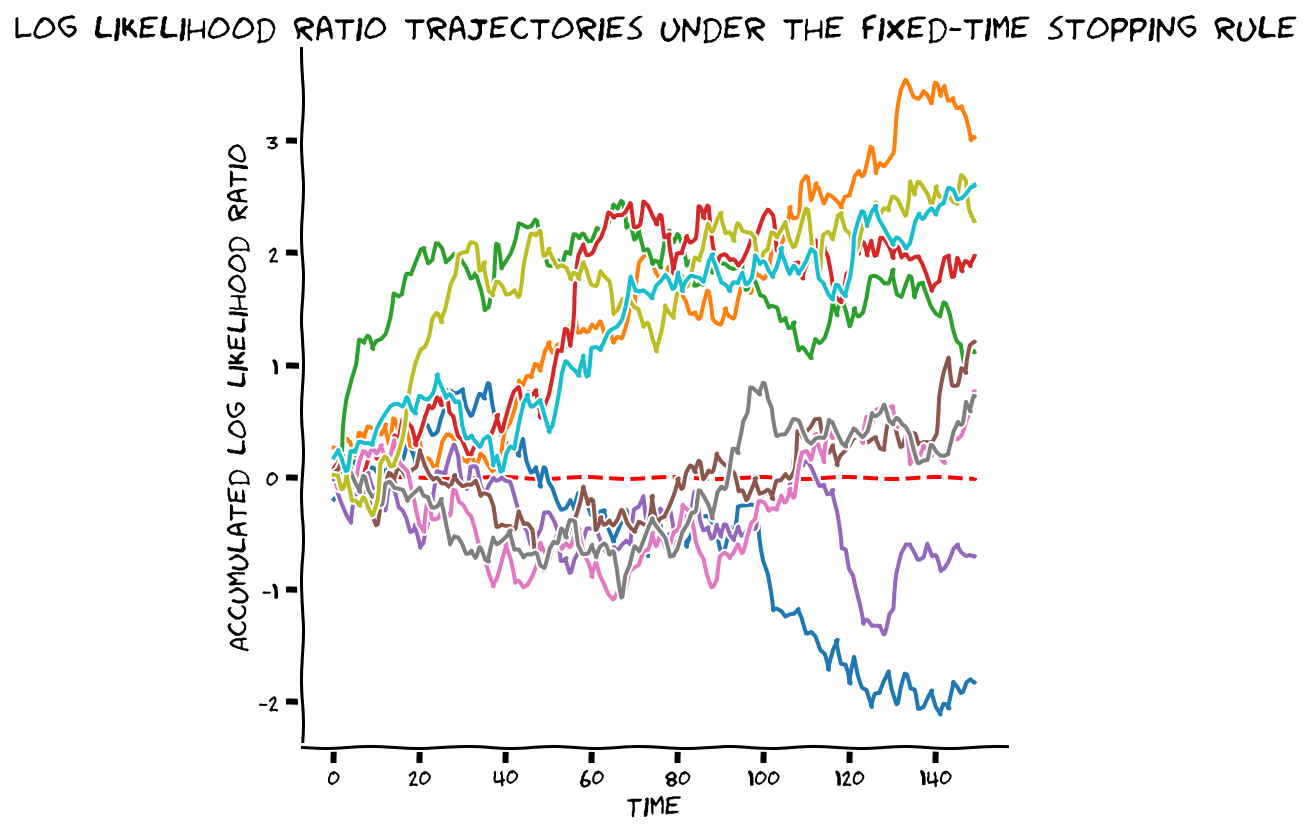
\includegraphics[scale=0.25]{Figures/HD/HD_Figure1.png}
\end{center}
Note:
\begin{enumerate}
    \item 
Higher noise, or higher sigma ($\sigma$), means that the evidence accumulation varies up
   and down more. You are more likely to make a wrong decision with high noise,
   since the accumulated log likelihood ratio is more likely to be negative at the end
   despite the true distribution being s = +1.

\item When sigma ($\sigma$) is very small, the cumulated log likelihood ratios are basically a linear
   diagonal line. This is because each new measurement will be very similar (since they are
   being drawn from a Gaussian with a tiny standard deviation)

\item You are more likely to be wrong with a small number of time steps before decision. There is
   more change that the noise will affect the decision. We will explore this in the next section.
\end{enumerate}

\end{subbox}
\end{textbox}
%%%%%%%%%%%%%%%%%%%%%%%%% 
%%%%%%%%%%%%%%%%%%%%%%%%%
\begin{textbox}{\href{https://compneuro.neuromatch.io/tutorials/W3D2_HiddenDynamics/student/W3D2_Tutorial1.html}{Sequential Probability Ratio Test }   }

\begin{subbox}{subbox}{Analyzing the DDM: accuracy vs stopping time}
\scriptsize

If you make a hasty decision (e.g., after only seeing 2 samples), or if observation noise buries the signal, you may see a negative accumulated log likelihood ratio and thus make a wrong decision. Let's plot how decision accuracy varies with the number of samples. Accuracy is the proportion of correct trials across our repeated simulations: $\frac{\# \textrm{ correct decisions}}{\# \textrm{ total decisions}}$.

\begin{center}
    
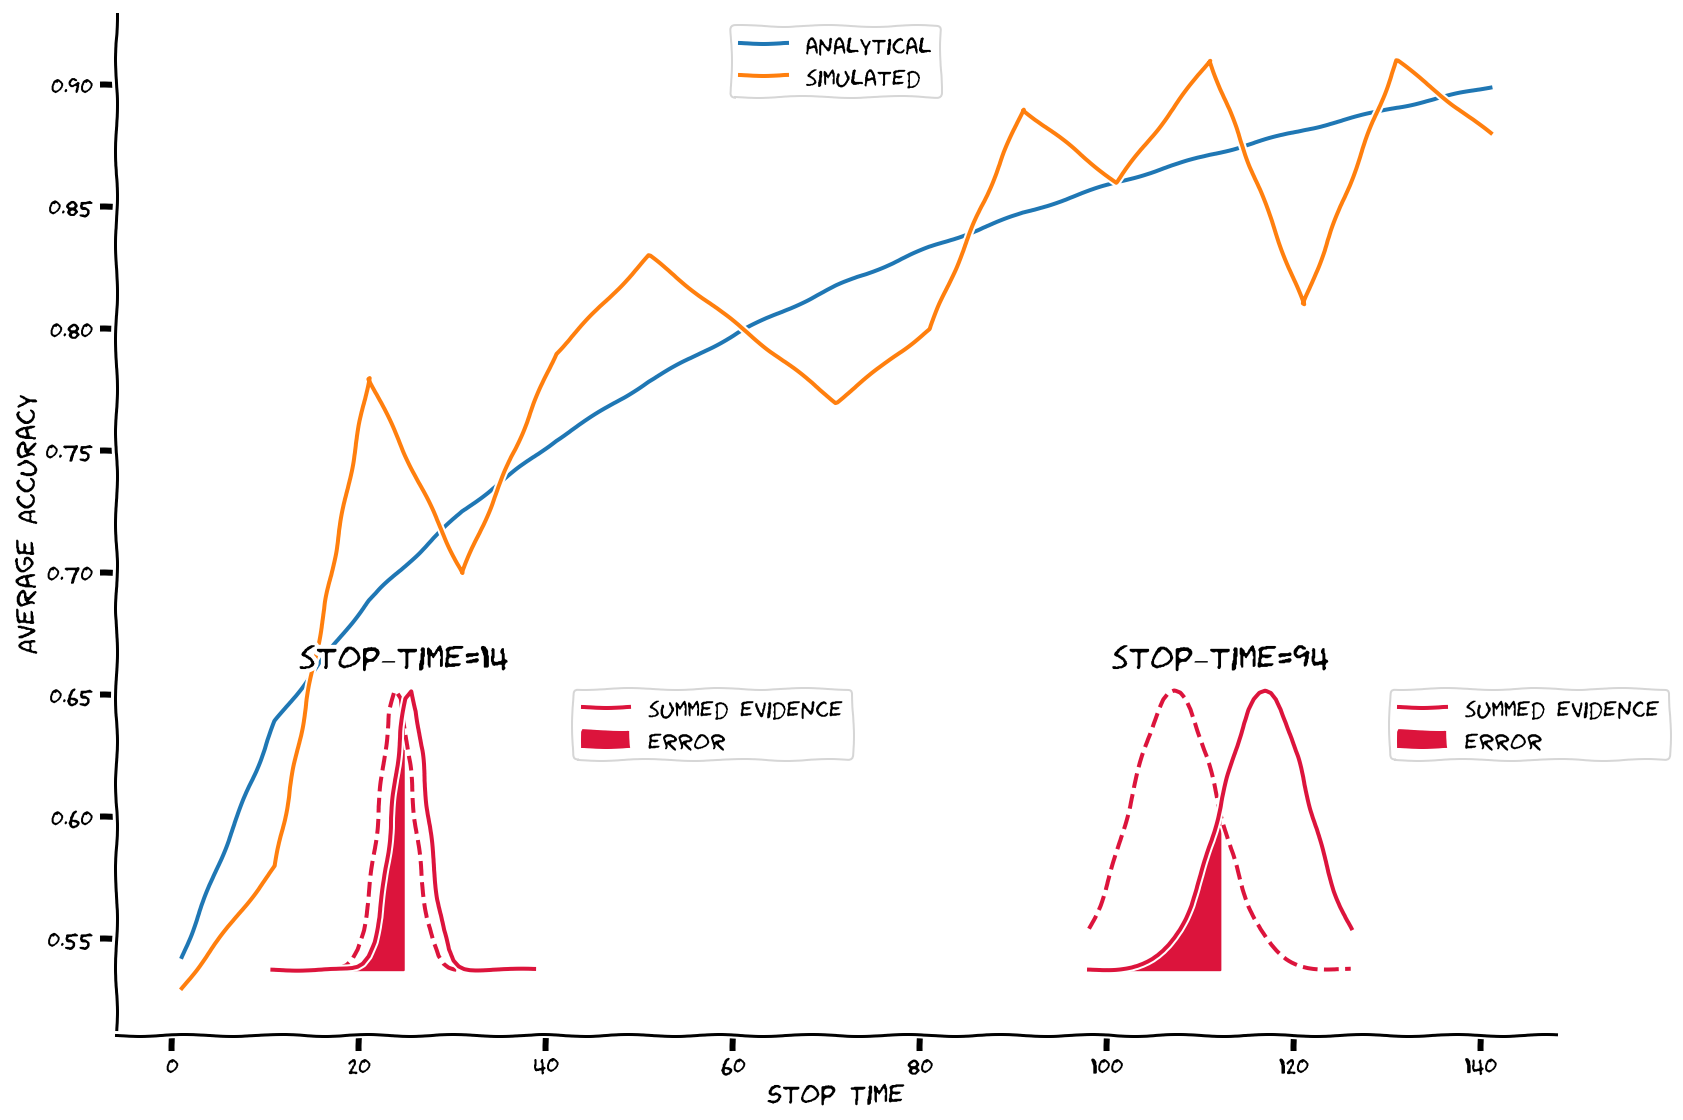
\includegraphics[scale=0.2]{Figures/HD/HD_Figure2.png}
\end{center}
In the figure above, we are plotting the simulated accuracies in orange. We can actually find an analytical equation for the average accuracy in this specific case, which we plot in blue. We will not dive into this analytical solution here but you can imagine that if you ran a bunch of different simulations and had the equivalent number of orange lines, the average of those would resemble the blue line. 

In the insets, we are showing the evidence distributions for the two states at a certain time point. Recall from Section 1 that the likelihood ratio at time $T$ for state of +1 is: 

\begin{equation}
L_T\sim\mathcal{N}\left(2\frac{\mu^2}{\sigma^2}T,\ 4\frac{\mu^2}{\sigma^2}T\right)=\mathcal{N}(bT,c^2T)
\end{equation}

If the state is -1, the mean is the reverse sign. We are plotting this Gaussian distribution for the state equaling -1 (dashed line) and the state equaling +1 (solid line). The area in red reflects the error rate - this region corresponds to $L_T$ being below 0 even though the true state is +1 so you would decide on the wrong state. As more time goes by, these distributions separate more and the error is lower.

\end{subbox}
\begin{subbox}{subbox}{Application}
\scriptsize


We have looked at the drift diffusion model of decisions in the context of the fishing problem. There are lots of uses of this in neuroscience! As one example, a classic experimental task in neuroscience is the random dot kinematogram \href{https://www.nature.com/articles/341052a0.pdf}{[Newsome, Britten, Movshon 1989]}, in which a pattern of moving dots are moving in random directions but with some weak coherence that favors a net rightward or leftward motion. The observer must guess the direction. Neurons in the brain are informative about this task, and have responses that correlate with the choice, as predicted by the Drift Diffusion Model (Huk and Shadlen 2005).

\end{subbox}
\end{textbox}
%%%%%%%%%%%%%%%%%%%%%%%%% 
%%%%%%%%%%%%%%%%%%%%%%%%%
%%% TUTORIAL 2
\newpage
%%%%%%%%%%%%%%%%%%%%%%%%% 
%%%%%%%%%%%%%%%%%%%%%%%%%
\begin{textbox}{\href{http://instructor.compneuro.neuromatch.io/tutorials/W3D2_HiddenDynamics/instructor/W3D2_Tutorial2.html}{Hidden Markov Model }   }

\begin{subbox}{subbox}{Application}
\scriptsize
The world around us is often changing, but we only have noisy sensory measurements. Similarly, neural systems switch between discrete states (e.g. sleep/wake) which are observable only indirectly, through their impact on neural activity. \textbf{Hidden Markov Models (HMM)} let us reason about these unobserved (also called hidden or latent) states using a time series of measurements. 

Here we'll learn how changing the HMM's transition probability and measurement noise impacts the data. We'll look at how uncertainty increases as we predict the future, and how to gain information from the measurements.

We will use a binary latent variable $s_t \in \{0,1\}$ that switches randomly between the two states, and a 1D Gaussian emission model $m_t|s_t \sim \mathcal{N}(\mu_{s_t},\sigma^2_{s_t})$ that provides evidence about the current state.

\end{subbox}
\begin{subbox}{subbox}{Binary HMM with Gaussian measurements}
\scriptsize

Here the latent state in an HMM is not fixed, but may switch to a different state at each time step. The time dependence is simple: the probability of the state at time $t$ is wholly determined by the state at time $t-1$. This is called called the \textbf{Markov property} and the dependency of the whole state sequence $\{s_1,...,s_t\}$ can be described by a chain structure called a Markov Chain. 

\end{subbox}
\begin{subbox}{subbox}{Markov model for binary latent dynamics}
\scriptsize

Let's reuse the binary switching process: our state can be either +1 or -1. The probability of switching to state $s_t=j$ from the previous state $s_{t-1}=i$ is the conditional probability distribution $p(s_t = j| s_{t-1} = i)$. We can summarize these as a $2\times 2$ matrix we will denote $D$ for Dynamics.

\begin{align*}
D = \begin{bmatrix}p(s_t = +1 | s_{t-1} = +1) & p(s_t = -1 | s_{t-1} = +1)\\p(s_t = +1 | s_{t-1} = -1)& p(s_t = -1 | s_{t-1} = -1)\end{bmatrix}
\end{align*}

$D_{ij}$ represents the transition probability to switch from state $i$ to state $j$ at next time step. 

We can represent the probability of the \textit{current} state as a 2-dimensional vector 

\begin{equation*}
P_t = [p(s_t = +1), p(s_t = -1)]
\end{equation*}

The entries are the probability that the current state is +1 and the probability that the current state is -1 so these must sum up to 1.

We then update the probabilities over time following the Markov process:

\begin{equation*}
P_{t}= P_{t-1}D 
\end{equation*}

If you know the state, the entries of $P_{t-1}$ would be either 1 or 0 as there is no uncertainty.

\textbf{Measurements}\\
In a \textit{Hidden Markov Model}, we cannot directly observe the latent states $s_t$. Instead we get noisy measurements $m_t\sim p(m|s_t)$.

\end{subbox}

\end{textbox}
%%%%%%%%%%%%%%%%%%%%%%%%% 
%%%%%%%%%%%%%%%%%%%%%%%%%
\begin{textbox}{\href{http://instructor.compneuro.neuromatch.io/tutorials/W3D2_HiddenDynamics/instructor/W3D2_Tutorial2.html}{Hidden Markov Model }   }

\begin{subbox}{subbox}{Simulate a binary HMM with Gaussian measurements}
\scriptsize
To implement a binary HMM with Gaussian measurements. Your HMM will start in State +1 and transition between states (both $-1 \rightarrow 1$ and $1 \rightarrow -1$) with probability switch probability. Each state emits measurements drawn from a Gaussian with mean $+1$ for State +1 and mean $-1$ for State -1. The standard deviation of both states is given by noise level.

To implement a binary HMM we have three steps:\\
\textbf{STEP 1}. Create the transition matrix  

\begin{equation}
D = 
\begin{pmatrix}
p_{\rm stay} & p_{\rm switch} \\
p_{\rm switch} & p_{\rm stay} \\
\end{pmatrix}
\end{equation}

with $p_{\rm stay} = 1 - p_{\rm switch}$. 

\textbf{STEP 2}. Specify gaussian measurements $m_t | s_t$, by specifying the means for each state, and the standard deviation.

\textbf{STEP 3}. Use the transition matrix to specify the probabilities for the next state $s_t$ given the previous state $s_{t-1}$.\\

The plot below shows an example HMM simulation. 
\begin{center}
    
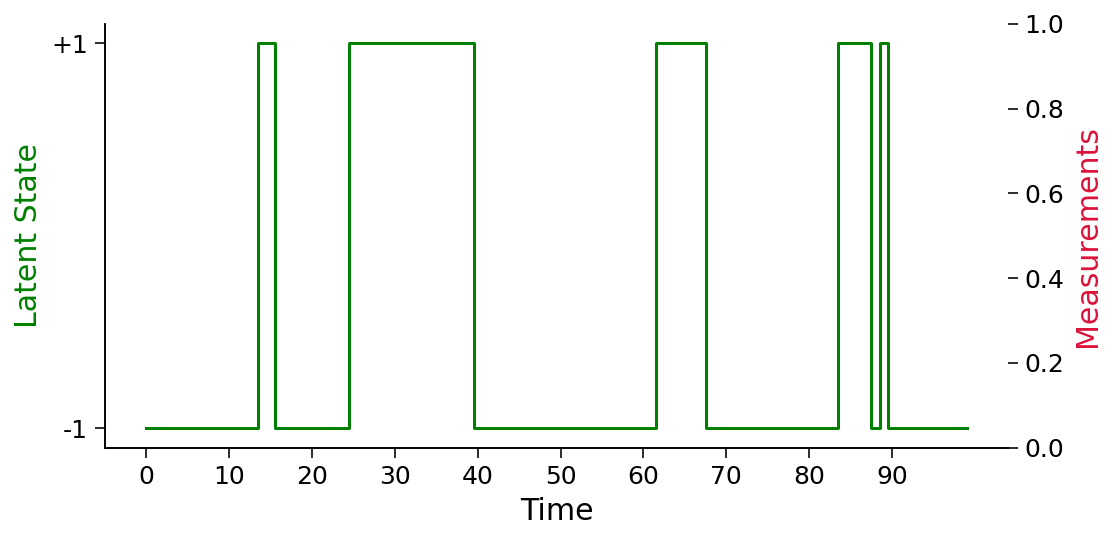
\includegraphics[scale=0.25]{Figures/HD/HD_Figure3.png}
\end{center}
\end{subbox}
\begin{subbox}{subbox}{Applications}
\scriptsize

Measurements could be:
\begin{itemize}
    \item 
 fish caught at different times as the school of fish moves from left to right
\item membrane voltage when an ion channel changes between open and closed
\item EEG frequency measurements as the brain moves between sleep stat
\end{itemize}

\end{subbox}
\begin{subbox}{subbox}{Forgetting in a changing world}
\scriptsize



Even if we know the world state for sure, the world changes. We become less and less certain as time goes by since our last measurement. We'll plot how a Hidden Markov Model gradually "forgets" the current state when predicting the future without measurements.
\begin{center}
    
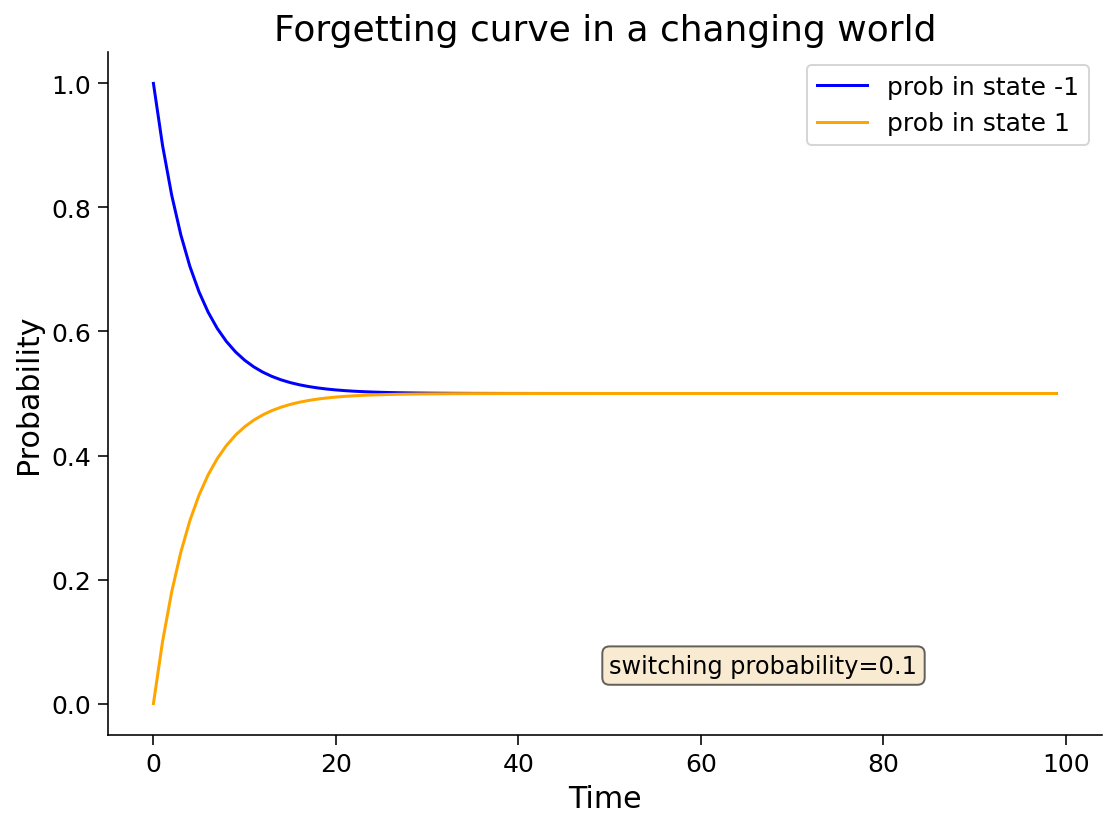
\includegraphics[scale=0.2]{Figures/HD/HD_Figure4.png}
\end{center}
\end{subbox}



\end{textbox}
%%%%%%%%%%%%%%%%%%%%%%%%% 
%%%%%%%%%%%%%%%%%%%%%%%%%
\begin{textbox}{\href{http://instructor.compneuro.neuromatch.io/tutorials/W3D2_HiddenDynamics/instructor/W3D2_Tutorial2.html}{Hidden Markov Model }   }

\begin{subbox}{subbox}{Forward inference of HMM}
\scriptsize
As a recursive algorithm, let's assume we already have yesterday's posterior from time $t-1$: $p(s_{t-1}|m_{1:t-1})$. When the new data $m_{t}$ comes in, the algorithm performs the following steps:\\

\textbf{Predict}: transform yesterday's posterior over $s_{t-1}$ into today's prior over $s_t$ using the transition matrix $D$:

\begin{equation*}
\text{today's prior}=p(s_t|m_{1:t-1})= p(s_{t-1}|m_{1:t-1}) D
\end{equation*}

\textbf{Update}: Incorporate measurement $m_t$ to calculate the posterior $p(s_t|m_{0:t})$

\begin{equation*}
\text{posterior} \propto \text{prior}\cdot \text{likelihood}=p(m_t|s_t)p(s_t|m_{0:t-1})
\end{equation*}


The plot below shows an example HMM simulation. 
\begin{center}
    
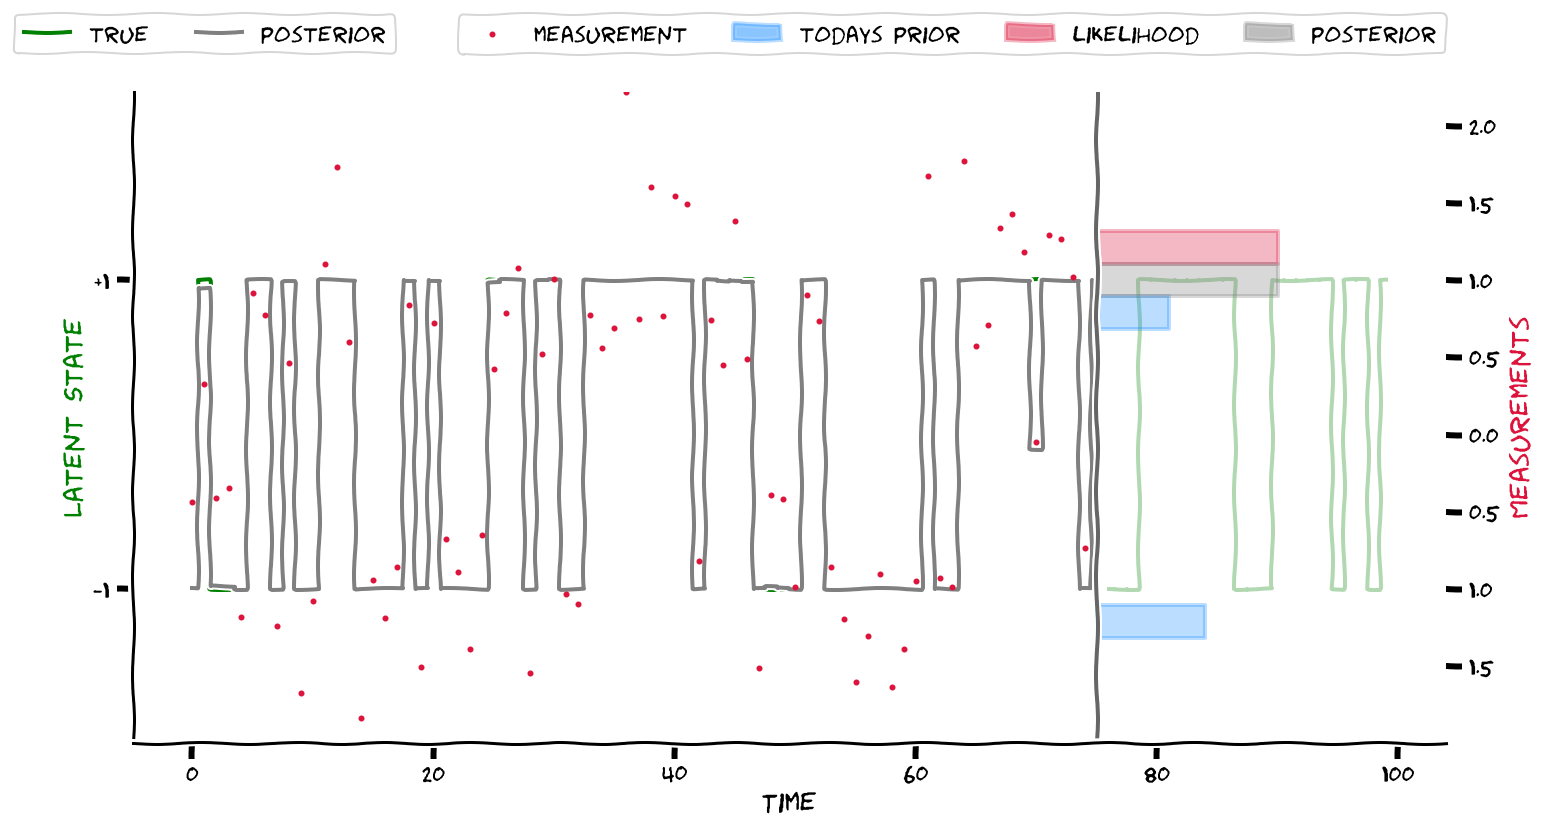
\includegraphics[scale=0.25]{Figures/HD/HD_Figure5.png}
\end{center}
\end{subbox}




\end{textbox}
%%%%%%%%%%%%%%%%%%%%%%%%% 
%%%%%%%%%%%%%%%%%%%%%%%%%
%%% TUTORIAL 3
\newpage
%%%%%%%%%%%%%%%%%%%%%%%%% 
%%%%%%%%%%%%%%%%%%%%%%%%%
\begin{textbox}{\href{http://instructor.compneuro.neuromatch.io/tutorials/W3D2_HiddenDynamics/instructor/W3D2_Tutorial3.html}{The Kalman Filter }   }

\begin{subbox}{subbox}{Application}
\scriptsize

We have used Hidden Markov Models (HMM) to infer \textit{discrete} latent states from a sequence of measurements. Here, we will learn how to infer a \textit{continuous} latent variable using the \textbf{Kalman filter}, which is one version of an HMM.

You can imagine this inference process happening as Mission Control tries to locate and track Astrocat. But you can also imagine that the brain is using an analogous Hidden Markov Model to track objects in the world, or to estimate the consequences of its own actions. And you could use this technique to estimate brain activity from noisy measurements, for understanding or for building a brain-machine interface.

\end{subbox}
\begin{subbox}{subbox}{Simulating Astrocat's movements}
\scriptsize
We will simulate how Astrocat moves based on stochastic linear dynamics.

The linear dynamical system 
$$ s_t = Ds_{t-1} + w_{t-1}$$
determines Astrocat's position $s_t$. $D$ is a scalar that models how Astrocat would like to change its position over time, and $w_t \sim \mathcal{N}(0, \sigma_p^2)$ is white Gaussian noise caused by unreliable actuators in Astrocat's propulsion unit. 

\begin{center}
    
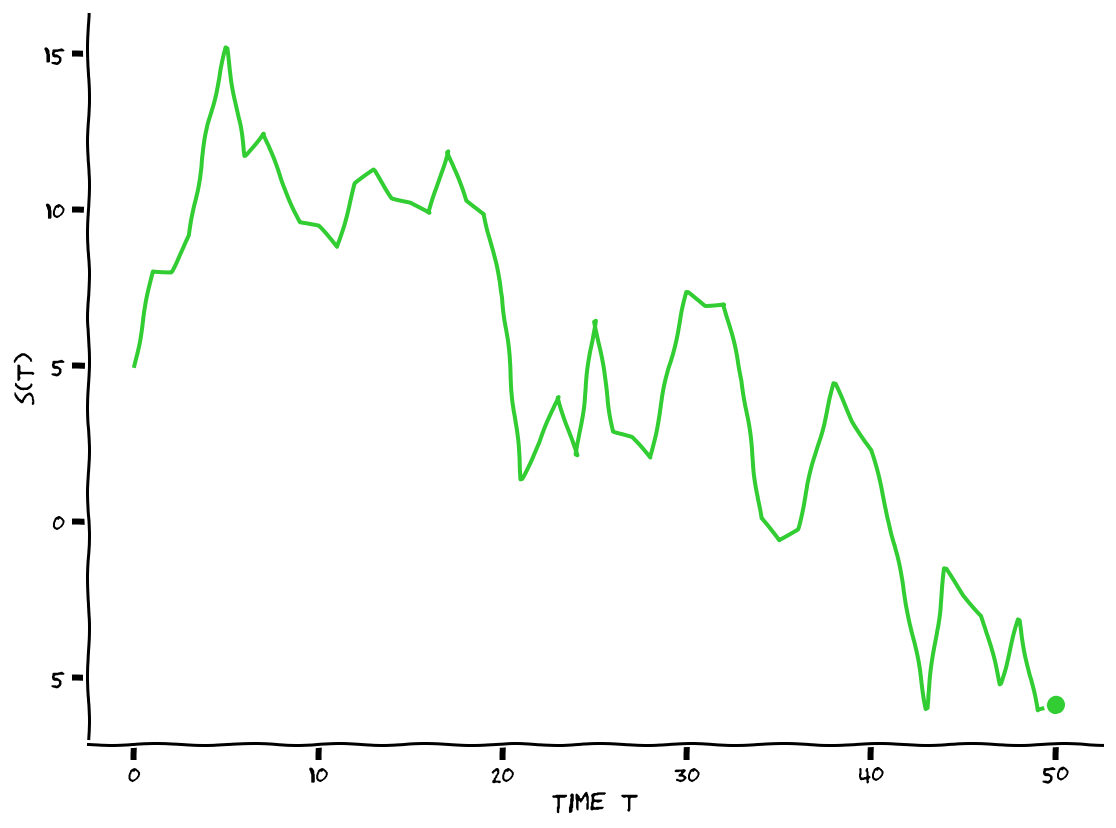
\includegraphics[scale=0.2]{Figures/HD/HD_Figure6.png}
\end{center}

\begin{enumerate}
    \item 
When D is large, the state at time step t will depend heavily on the state at time
   step $t_1$. If we forget about the noise term, D = 2 would mean that the state at each
   time step is double the one before! So the state becomes huge and basically explodes towards
   infinity.

\item If D is a large negative number, the state at time t will be a different sign than the
   state at time step $t_1$. So the state will oscillate over the x axis.

\item When D is zero, the state at time t will not depend on the previous state, it will just
   be drawn from the noise distribution.
   \end{enumerate} 
\end{subbox}

\end{textbox}
%%%%%%%%%%%%%%%%%%%%%%%%% 
%%%%%%%%%%%%%%%%%%%%%%%%%
\begin{textbox}{\href{http://instructor.compneuro.neuromatch.io/tutorials/W3D2_HiddenDynamics/instructor/W3D2_Tutorial3.html}{The Kalman Filter }   }

\begin{subbox}{subbox}{Implementing a Kalman filter}
\scriptsize

A Kalman filter estimates a posterior probability distribution \textit{recursively} over time using a mathematical model of the process and incoming measurements. This dynamic posterior allows us to improve our guess about Astrocat's position as new measures arrive; besides, its mean is the best estimate one can compute of Astrocat's actual position at each time step.

Follow this recipe to implement your own Kalman filter:

\textbf{Step 1: Change yesterday's posterior into today's prior}\\

Use the mathematical model to calculate how deterministic changes in the process shift yesterday's posterior, $\mathcal{N}(\mu_{s_{t-1}}, \sigma_{s_{t-1}}^2)$, and how random changes in the process broaden the shifted distribution:

\begin{align*}
p(s_t|m_{1:t-1}) &=& p(Ds_{t-1}+w_{t-1} | m_{1:t-1})\\ 
&=& \mathcal{N}(D\mu_{s_{t-1}} + 0, D^2\sigma_{s_{t-1}}^2 +\sigma_p^2)
\end{align*}

Note that we use $\sigma_p$ here to denote the process noise.

\textbf{Step 2: Multiply today's prior by likelihood} \\

Use the latest measurement of Astrocat's collar (fresh evidence) to form a new estimate somewhere between this measurement and what we predicted in Step 1. The next posterior is the result of multiplying the Gaussian computed in Step 1 (a.k.a. today's prior) and the likelihood, which is also modeled as a Gaussian $\mathcal{N}(m_t, \sigma_m^2)$:

\texbf{Step 2a: add information from prior and likelihood}\\

To find the posterior variance, we first compute the posterior information (which is the inverse of the variance) by adding the information provided by the prior and the likelihood:

\begin{equation}
\frac{1}{\sigma_{s_t}^2} = \frac{1}{D^2\sigma_{s_{t-1}}^2 +\sigma_p^2} + \frac{1}{\sigma_m^2}
\end{equation}

Now we can take the inverse of the posterior information to get back the posterior variance.

\textbf{Step 2b: add means from prior and likelihood}\\ 

To find the posterior mean, we calculate a weighted average of means from prior and likelihood, where each weight, $g$, is just the fraction of information that each Gaussian provides!

\begin{align}
g_{\rm{prior}} &= \frac{\rm{information}_{\textit{ }\rm{prior}}}{\rm{information}_{\textit{ }\rm{posterior}}} \\
g_{\rm{likelihood}} &= \frac{\rm{information}_{\textit{ }\rm{likelihood}}}{\rm{information}_{\textit{ }\rm{posterior}}} \\
\bar{\mu}_t &= g_{\rm{prior}} D\mu_{s_{t-1}} + g_{\rm{likelihood}} m_t
\end{align}
\end{subbox}

\end{textbox}
%%%%%%%%%%%%%%%%%%%%%%%%% 
%%%%%%%%%%%%%%%%%%%%%%%%%
\begin{textbox}{\href{http://instructor.compneuro.neuromatch.io/tutorials/W3D2_HiddenDynamics/instructor/W3D2_Tutorial3.html}{The Kalman Filter }   }

\begin{subbox}{subbox}{Relationship to classic description of Kalman filter}
\scriptsize

We're teaching this recipe because it is interpretable and connects to past lessons about the sum rule and product rule for Gaussians. But the classic description of the Kalman filter is a little different. The above weights, $g_{\rm{prior}}$ and $g_{\rm{likelihood}}$, add up to $1$ and can be written one in terms of the other; then, if we let $K = g_{\rm{likelihood}}$, the posterior mean can be expressed as:

\begin{equation}
\bar{\mu}_t = (1-K) D\bar{\mu}_{t-1} + K m_t = D\bar{\mu}_{t-1} + K (m_t - D\bar{\mu}_{t-1})
\end{equation}

In classic textbooks, you will often find this expression for the posterior mean; $K$ is known as the Kalman gain and its function is to choose a value partway between the current measurement $m_t$ and the prediction from Step 1.


\begin{center}
    
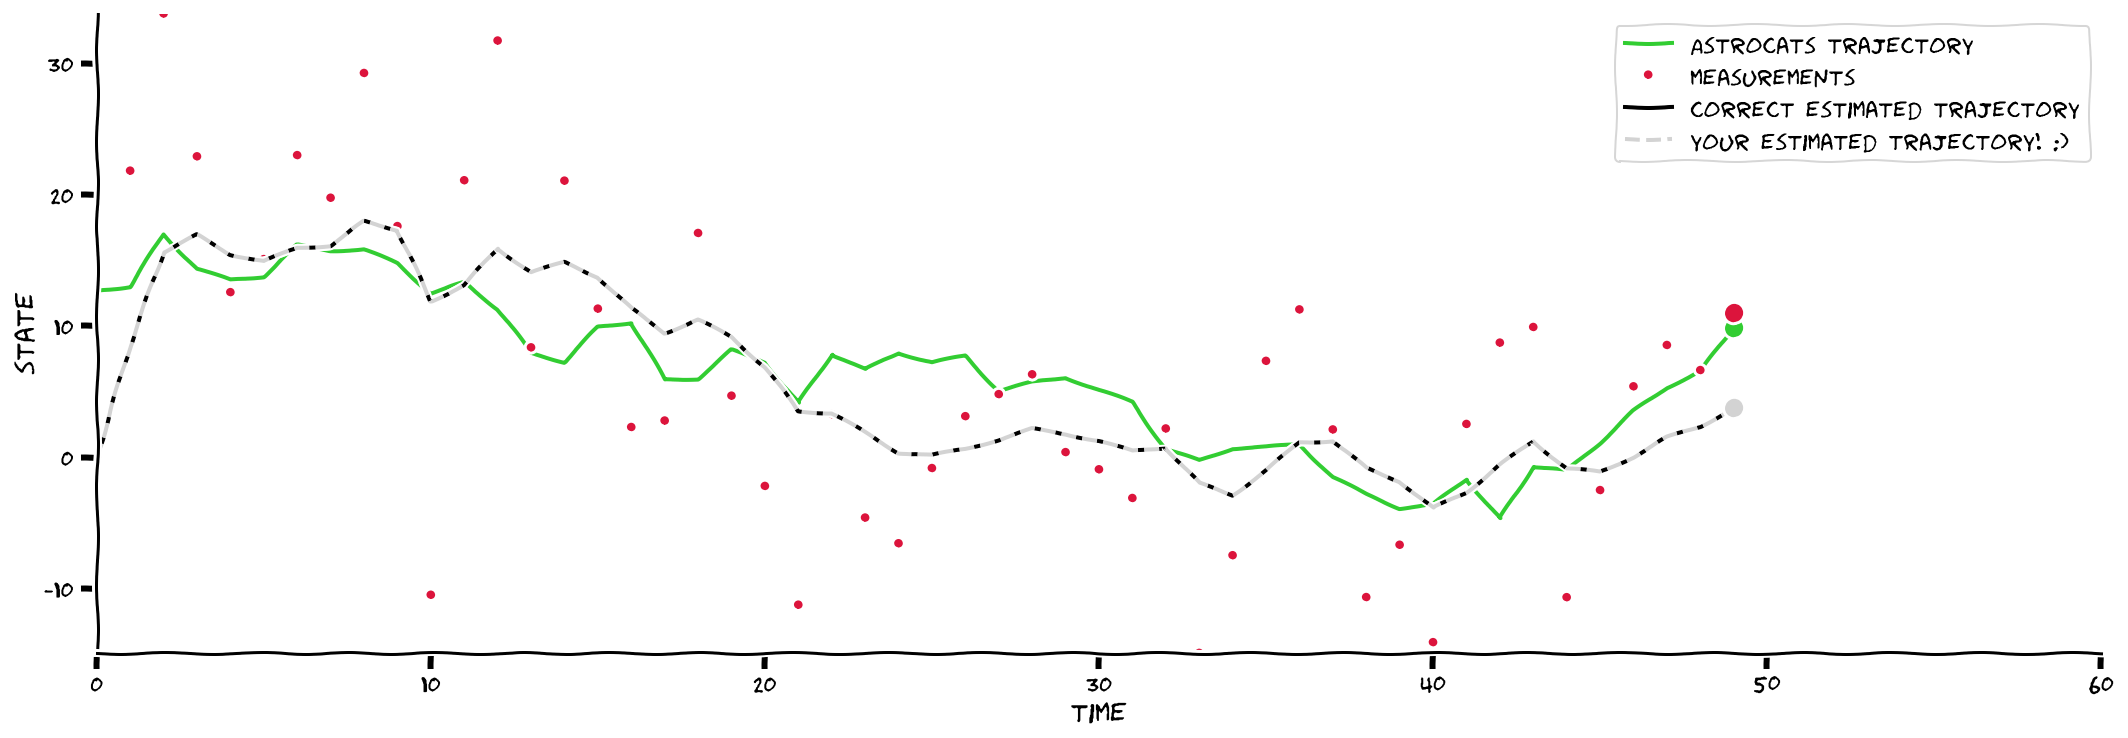
\includegraphics[scale=0.17]{Figures/HD/HD_Figure7.png}
\end{center}

\end{subbox}
\begin{subbox}{subbox}{Compare states, estimates, and measurements}
\scriptsize

How well do the estimates $\hat{s}$ match the actual values $s$? How does the distribution of errors $\hat{s}_t - s_t$ compare to the posterior variance? Why? Try different parameters of the Hidden Markov Model and observe how the properties change.

How do the measurements $m$ compare to the true states?


\begin{center}
    
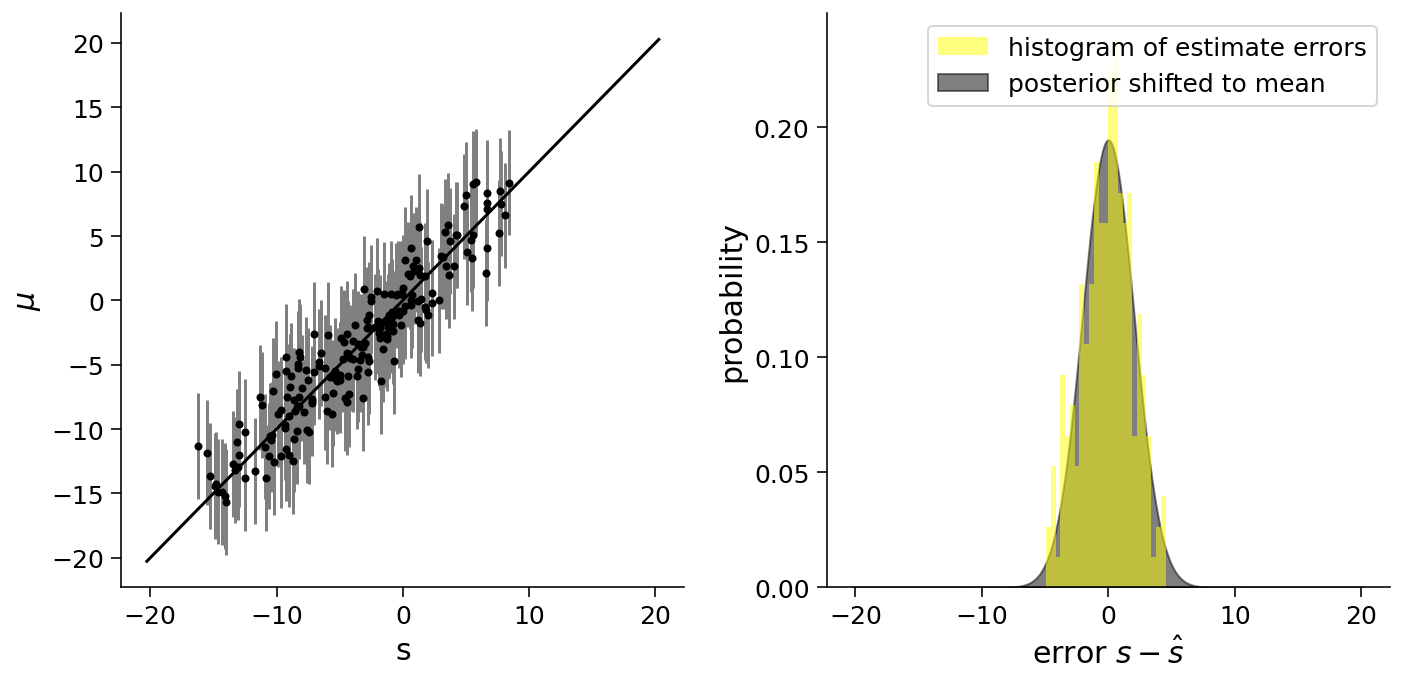
\includegraphics[scale=0.27]{Figures/HD/HD_Figure8.png}
\end{center}

\end{subbox}
\end{textbox}
%%%%%%%%%%%%%%%%%%%%%%%%% 
%%%%%%%%%%%%%%%%%%%%%%%%%
\begin{textbox}{\href{http://instructor.compneuro.neuromatch.io/tutorials/W3D2_HiddenDynamics/instructor/W3D2_Tutorial3.html}{The Kalman Filter }   }

\begin{subbox}{subbox}{ How long does it take to find astrocat?}
\scriptsize

Here we plot the posterior variance as a function of time. Before mission control gets measurements, their only information about astrocat's location is the prior. After some measurements, they hone in on astrocat.
\begin{itemize}
    \item 
 How does the variance shrink with time?
\item The speed depends on the process dynamics, but does it also depend on the signal-to-noise ratio (SNR)? (Here we measure SNR in decibels, a log scale where 1 dB means 0.1 log unit.)
\end{itemize}

The red curve shows how rapidly the latent variance equilibrates exponentially from an initial condition, with a time constant of $\sim 1/(1-D^2)$. 

\begin{center}
    
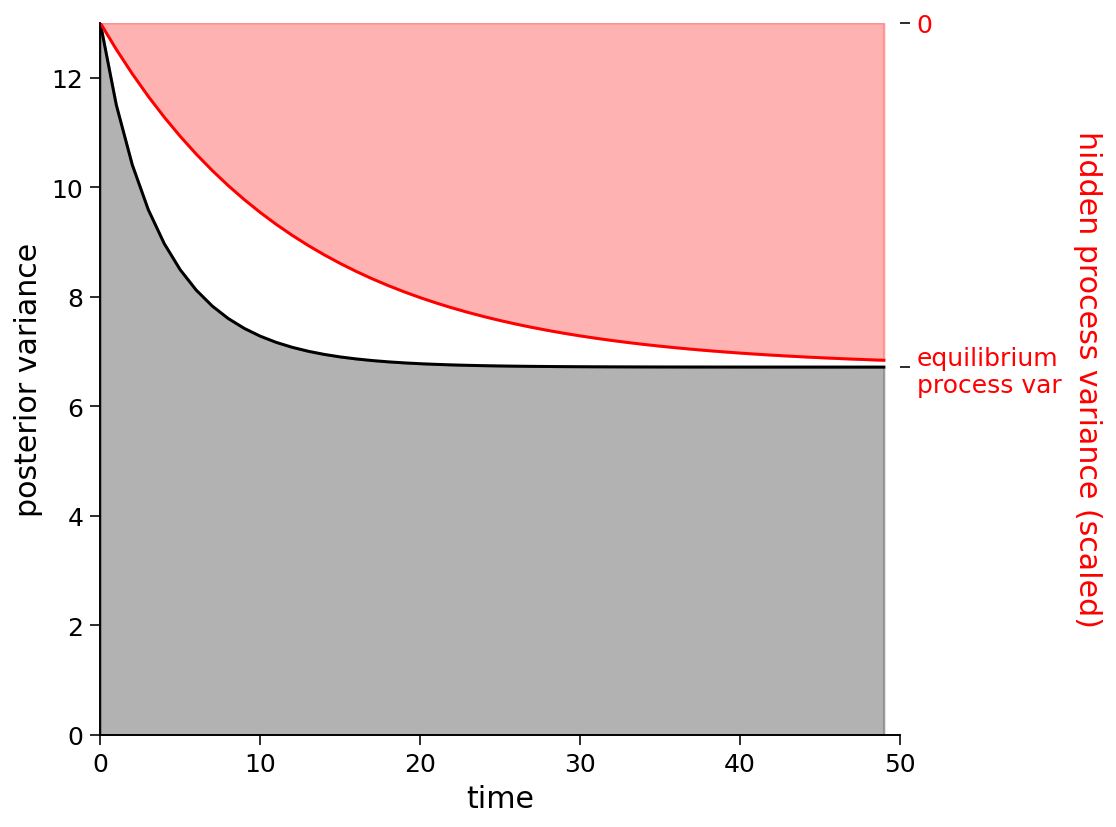
\includegraphics[scale=0.25]{Figures/HD/HD_Figure9.png}
\end{center}

\end{subbox}
\begin{subbox}{subbox}{ Applications of Kalman filter in brain science}
\scriptsize


\begin{itemize}
    \item  Brain-Computer Interface: estimate intended movements using neural activity as measurements.
\item Data analysis: estimate brain activity from noisy measurements (e.g., EEG)
\item Model of perception: prey tracking using noisy sensory measurements
\item Imagine your own! When are you trying to estimate something you cannot see directly?
\end{itemize}
There are many variants that improve upon the limitations of the Kalman filter: non-Gaussian states and measurements, nonlinear dynamics, and more.

\end{subbox}
\end{textbox}
